\documentclass{zc-ust-hw}

% Shared by every phase report: packages, title block, team, repository link.
\usepackage{booktabs}
\usepackage{microtype}
\hypersetup{colorlinks=true, linkcolor=black, citecolor=black, urlcolor=blue!60!black}
\lstset{language=C++, numbers=none, basicstyle=\ttfamily\footnotesize}
\setlist{itemsep=2pt, topsep=4pt}

% Title block: name / ID / date in a wrapping column beside the logo, so long name or ID
% lists continue on the next line instead of running under the logo.
\makeatletter
\renewcommand{\maketitle}{%
  \noindent
  \begin{minipage}[t]{0.76\linewidth}
    \vspace{0pt}
    \begin{tabular}[t]{@{}l p{0.82\linewidth}@{}}
      \ifx\@name\empty\else Name: & \raggedright \@name \tabularnewline \fi
      \ifx\@id\empty\else ID: & \raggedright \@id \tabularnewline \fi
      Date: & \today
    \end{tabular}
  \end{minipage}\hfill
  \begin{minipage}[t]{0.2\linewidth}
    \vspace{0pt}\raggedleft
    
\includegraphics[height=2cm]{logo.jpg}
  \end{minipage}

  \begin{center}
    \textbf{\large \@course}\\
    \@assignment
  \end{center}

  \noindent\rule{\linewidth}{0.1mm}
  \medskip
}
\makeatother

\newcommand{\repo}{\url{https://github.com/AliAshraf69420/Parallel-Distributed-Project}}

\name{Ali Ashraf Hassan Abdelghany, Ahmad Muhammadi, Omar Ali, Abdullah Ayman}
\id{202301812, 202301826, 202300942, 202301731}
\course{SW 401}

\graphicspath{{../plots/phase2/}}
\assignment{Phase 2 Report: Scaling Across Nodes (MPI)}

\begin{document}

\maketitle

\noindent\textbf{Repository:} \repo\ (MPI code in \texttt{src/mpi/}, run scripts and hostfile
in \texttt{scripts/mpi/}).\\
\textbf{Environments.} \emph{Host}: one machine (Ryzen 7 5800H, 8 cores), OpenMPI 5.0.11,
\texttt{mpirun --bind-to core}, shared-memory transport. \emph{Cluster}: four Docker containers on
that machine, each pinned to 2 separate physical cores, joined by a bridge network; ranks in
different containers communicate over TCP, ranks in the same container over shared memory.
Ranks are placed round-robin, so $P=2$ already crosses the network.

%======================================================================
\section{Design: decomposition and data flow}
%======================================================================

The computation is unchanged from Phase 1: crop and resize every image to $224\times224$,
compute the per-channel mean and standard deviation over the training images (pass 1), then
normalize every image (pass 2). Every MPI run is checked bit for bit against the same
reference as the sequential and OpenMP versions, and every run in this report passed.

\begin{figure}[H]
\centering
\begin{tikzpicture}[font=\footnotesize,
  box/.style={draw, rounded corners=2pt, minimum height=9mm, minimum width=34mm, align=center, fill=gray!8},
  bar/.style={draw, rounded corners=2pt, minimum height=7mm, minimum width=132mm, align=center, fill=blue!8},
  file/.style={draw, dashed, minimum height=6mm, align=center, fill=yellow!12},
  arr/.style={-{Stealth[length=2mm]}, semithick}]
  % row a: index distribution
  \node[file] (idx) at (-0.75,1.3) {\texttt{index.bin}};
  \node[box] (a0) at (0,0) {\textbf{Rank 0}\\read index, cut $P$ blocks};
  \node[box] (a1) at (4.7,0) {\textbf{Rank 1}\\receive its records};
  \node at (7.35,0) {$\cdots$};
  \node[box] (ap) at (10,0) {\textbf{Rank $P{-}1$}\\receive its records};
  \draw[arr] (idx) -- (idx |- a0.north);
  \draw[arr] (a0) -- node[above, font=\scriptsize] {\texttt{MPI\_Send}} (a1);
  \draw[arr] ([xshift=-6mm]a0.north east) to[bend left=13] node[above, pos=0.55, font=\scriptsize]
        {\texttt{MPI\_Send}} ([xshift=6mm]ap.north west);
  % row b: pass 1
  \node[box] (b0) at (0,-1.55) {map own shards\\pass 1: private \texttt{Stats}};
  \node[box] (b1) at (4.7,-1.55) {map own shards\\pass 1: private \texttt{Stats}};
  \node at (7.35,-1.55) {$\cdots$};
  \node[box] (bp) at (10,-1.55) {map own shards\\pass 1: private \texttt{Stats}};
  \node[bar] (r1) at (5,-2.95) {\texttt{MPI\_Allreduce}(7 $\times$ \texttt{uint64}, \texttt{MPI\_SUM}):
      every rank now holds the global $\mu$, $\sigma$ and lookup table};
  % row c: pass 2
  \node[box] (c0) at (0,-4.35) {pass 2: normalize\\own records, CRCs};
  \node[box] (c1) at (4.7,-4.35) {pass 2: normalize\\own records, CRCs};
  \node at (7.35,-4.35) {$\cdots$};
  \node[box] (cp) at (10,-4.35) {pass 2: normalize\\own records, CRCs};
  \node[bar] (r2) at (5,-5.75) {\texttt{MPI\_Gatherv}(CRCs, 2 $\times$ 5.8 KiB per rank) and
      \texttt{MPI\_Gather}(timings) to rank 0};
  \node[file] (out) at (0,-7.0) {\texttt{stats.json}, \texttt{checksums.csv}};
  \node[file] (sh) at (7.6,-7.0) {\texttt{shard\_*.bin} (5.9 GiB): read by each rank, never sent};
  \foreach \x/\a/\b/\c in {0/a0/b0/c0, 4.7/a1/b1/c1, 10/ap/bp/cp} {
    \draw[arr] (\a) -- (\b);
    \draw[arr] (\b) -- (\b |- r1.north);
    \draw[arr] (\c |- r1.south) -- (\c);
    \draw[arr] (\c) -- (\c |- r2.north);
  }
  \draw[arr] (c0 |- r2.south) -- (out);
\end{tikzpicture}
\caption{Data flow. Each \texttt{MPI\_Send} carries a 24-byte header and that rank's block of
32-byte records (46\,KiB at $P=8$; the whole index is 368\,KiB). Only metadata and results
travel through MPI, about 0.4\,MiB in total for the full set at $P=8$. The 5.9\,GiB of pixels
is read by the rank that processes it.}
\label{fig:flow}
\end{figure}

\paragraph{Decomposition.} A one-dimensional block partition of the records, in storage order.
Images are independent, so there is no halo exchange, and a contiguous block keeps each rank's
file reads sequential. Rank 0 is the only rank that reads the index. It sends every rank its
block of records with \texttt{MPI\_Send} (point-to-point), and each rank maps only the shards
its records live in. We chose ``move the work to the data'' because the pixels are 14{,}000
times larger than everything that must be communicated.

\paragraph{What to balance.} The \texttt{--partition} option cuts the blocks to equalize record
count, source pixels, or estimated work (every record is normalized; training records are also
resized in pass 1). Phase 1 showed that the cost per image is uniform, because the resize cost
depends on the fixed output size. The measurements agree (Table~\ref{tab:part}): balancing
records or work keeps ranks within 2--4\,\% of each other, while balancing pixels (I/O volume)
gives 9\,\% imbalance and the slowest run. We use \texttt{work} by default.

\begin{table}[H]
\centering\small
\begin{tabular}{lrrrrr}
\toprule
Balance & Records/rank & MiB/rank & Rank time (s) & Imbalance & Total (s) \\
\midrule
work (default) & 1458--1477 & 730--771 & 1.348--1.397 & 3.5\,\% & 1.409 \\
count & 1473--1474 & 738--769 & 1.336--1.363 & 2.0\,\% & 1.403 \\
pixels & 1448--1511 & 755--756 & 1.327--1.459 & 9.1\,\% & 1.454 \\
\bottomrule
\end{tabular}
\caption{Per-rank balance at $P=8$ on the full set (host). Imbalance = (max $-$ min)/max of each
rank's pass 1 + pass 2 time.}
\label{tab:part}
\end{table}

\paragraph{Collectives.} Pass 1 ends with one \texttt{MPI\_Allreduce} over seven 64-bit
counters. Because the counters are exact integer sums, the result is identical for any $P$ and
any partition, and the call doubles as the barrier between the passes. Results return with
\texttt{MPI\_Gatherv} (per-image CRCs, variable counts per rank) and \texttt{MPI\_Gather}
(per-rank timings). With \texttt{--write}, each rank writes its own blocks of the output file
with \texttt{pwrite}; nothing is funnelled through rank 0.

%======================================================================
\section{Latency and bandwidth}
%======================================================================

\texttt{src/mpi/pingpong.cpp} measures the round-trip time (RTT) between two ranks for messages
from 1\,B to 64\,MiB (median of up to 2000 round trips per size, Figure~\ref{fig:pp}).

\begin{table}[H]
\centering\small
\begin{tabular}{lrrrrr}
\toprule
Setting & Latency & Bandwidth & RTT 64\,B & RTT 512\,KiB & RTT 64\,MiB \\
\midrule
Host, shared memory & 0.22\,\textmu s & 32.1\,GB/s & 0.47\,\textmu s & 50\,\textmu s & 16.1\,ms \\
Container, same node & 0.21\,\textmu s & 28.4\,GB/s & 0.34\,\textmu s & 43\,\textmu s & 13.6\,ms \\
Across nodes (TCP) & 6.37\,\textmu s & 7.6\,GB/s & 12.5\,\textmu s & 181\,\textmu s & 21.5\,ms \\
\bottomrule
\end{tabular}
\caption{Ping-pong summary. Latency is one-way: half the median RTT of messages up to 64\,B.
Bandwidth is the best $2\times\text{bytes}/\text{RTT}$ over all sizes.}
\end{table}

Across nodes the RTT is flat at 12.5\,\textmu s up to about 1\,KiB: this is the
\textbf{latency-dominated} region, where the cost is the TCP stack and the size does not matter.
Above about 64\,KiB the RTT grows in proportion to the size: the
\textbf{bandwidth-dominated} region. Shared memory is 30 times faster for small messages, and
shows a step at 4\,KiB where OpenMPI switches from eager to rendezvous delivery.

\emph{Relating this to our messages.} The \texttt{Allreduce} payload is 56\,B, deep in the
latency region: it costs microseconds regardless of transport. The record blocks (46\,KiB) and
CRC arrays (5.8\,KiB) are sent once per run. In total the application exchanges about 0.4\,MiB
to process 5.9\,GiB. On rank 0, the \texttt{Allreduce} (including waiting for the slowest rank
to finish pass 1) takes 26\,\textmu s on the host and 0.85\,ms on the cluster, against a 1.4\,s
run. Communication is below 0.1\,\% of the run time, which is why the cluster scales like the
host (Section~\ref{sec:scaling}). A normalized tensor, in contrast, is 588\,KiB, in the
bandwidth region: about 25\,\textmu s one way in shared memory and 90\,\textmu s over TCP,
against 640\,\textmu s to compute it. That is the message used in the next experiment.

\begin{figure}[H]
\centering
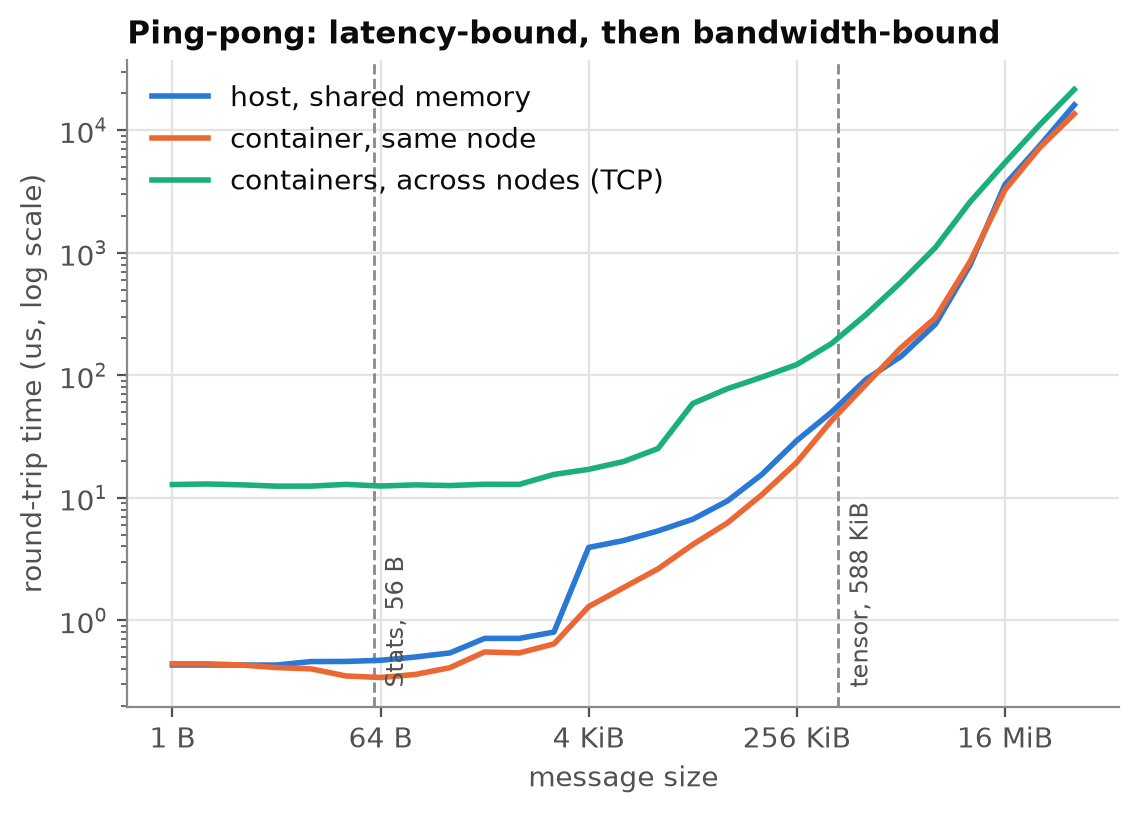
\includegraphics[width=0.6\linewidth]{pingpong.png}
\caption{Round-trip time against message size, with our two characteristic message sizes.}
\label{fig:pp}
\end{figure}

%======================================================================
\section{Overlapping communication and computation}
%======================================================================

To study a communication step that matters, \texttt{--collect} changes the design to the common
``workers send results to a master'' pattern: rank 0 only collects, and ranks $1..P{-}1$ ship
every normalized tensor to it (971 tensors, 558\,MiB, on the 500MB set). Rank 0 verifies the
CRC of every tensor it receives, so this path is checked end to end as well.
\begin{itemize}
  \item \texttt{send}: compute tensor $k$, \texttt{MPI\_Send} it, then compute tensor $k+1$.
  \item \texttt{isend}: \texttt{MPI\_Isend} tensor $k$, compute tensor $k+1$ into a second
    buffer, then \texttt{MPI\_Wait} before reusing the first. We call \texttt{MPI\_Test} between
    the kernels, because OpenMPI only advances a large transfer inside MPI calls.
\end{itemize}

\begin{table}[H]
\centering\small
\begin{tabular}{rrrrrrr}
\toprule
 & \multicolumn{3}{c}{Host (shared memory)} & \multicolumn{3}{c}{Cluster (TCP)} \\
\cmidrule(lr){2-4}\cmidrule(lr){5-7}
Workers & send (ms) & isend (ms) & hidden & send (ms) & isend (ms) & hidden \\
\midrule
1 & 44.1 & 0.5 & 99\,\% & 150.1 & 7.2 & 95\,\% \\
2 & 22.8 & 0.3 & 99\,\% & 95.4 & 73.1 & 23\,\% \\
3 & 55.4 & 59.8 & none & 126.1 & 168.5 & none \\
7 & 181.4 & 203.5 & none & 263.9 & 284.0 & none \\
\bottomrule
\end{tabular}
\caption{Mean time one worker spends inside \texttt{MPI\_Send}, or inside
\texttt{MPI\_Wait}+\texttt{MPI\_Isend}, over the run. Hidden $= 1 - \text{isend}/\text{send}$.}
\label{tab:overlap}
\end{table}

\begin{figure}[H]
\centering
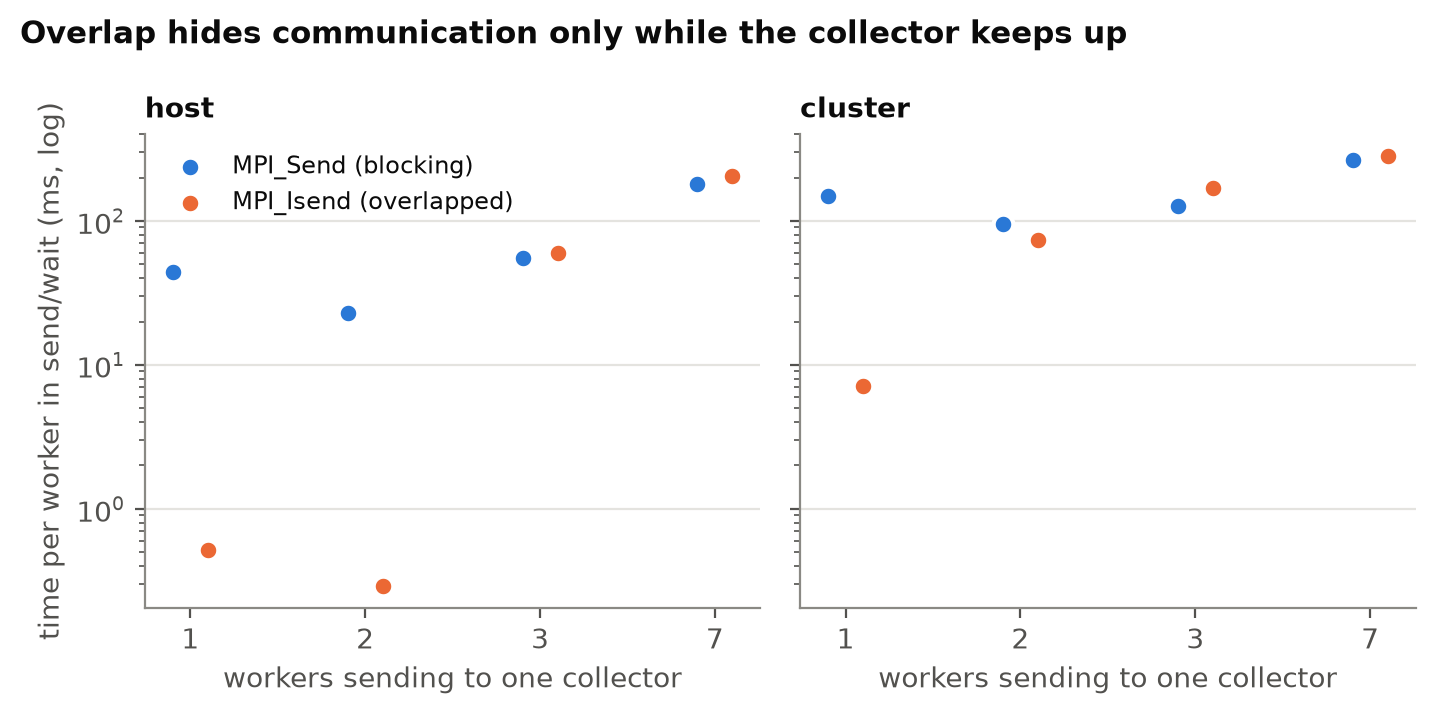
\includegraphics[width=0.78\linewidth]{overlap.png}
\caption{The values of Table~\ref{tab:overlap} (log scale).}
\label{fig:overlap}
\end{figure}

With one worker, a blocking send costs 45\,\textmu s per tensor in shared memory and
155\,\textmu s over TCP, consistent with the ping-pong. \textbf{Overlapping hides 95--99\,\% of
it}: the transfer completes while the next image is computed, and pass 2 gets 2--8\,\% faster.
\textbf{The benefit disappears once the collector is saturated.} Rank 0 can receive and verify
about 3{,}300 tensors per second (1.9\,GiB/s), which two to three workers already produce. From
then on workers wait for rank 0, not for the wire, and a non-blocking send cannot hide waiting
for a busy receiver; pass 2 stays near 0.30\,s however many workers are added. The same
500MB set takes 0.11\,s at $P=8$ in the normal design, where every rank writes its own output.
This is Amdahl's law applied to a serial collector, and it is the reason the main design has no
master in the data path.

%======================================================================
\section{Scaling study}\label{sec:scaling}
%======================================================================

Method as in Phase 1: one warm-up and three measured runs per configuration, median reported,
data preloaded. $T_S$ is the Phase 1 sequential time (9.79\,s compute, 10.06\,s total on the
full set). ``Compute'' is pass 1 + \texttt{Allreduce} + pass 2 as wall-clock time on rank 0;
``total'' adds distributing the index, opening the shards and writing the results.

\begin{table}[H]
\centering\small
\begin{tabular}{rrrrrrrrrr}
\toprule
 & \multicolumn{4}{c}{MPI, host} & \multicolumn{3}{c}{MPI, cluster} & \multicolumn{2}{c}{OpenMP} \\
\cmidrule(lr){2-5}\cmidrule(lr){6-8}\cmidrule(lr){9-10}
$P$ & compute (s) & $S$ & $E$ & $S_\text{total}$ & compute (s) & $S$ & $S_\text{total}$ & $S$ & $S_\text{total}$ \\
\midrule
1 & 9.486 & 1.03 & 1.03 & 1.03 & 9.454 & 1.04 & 1.03 & 1.01 & 1.01 \\
2 & 4.890 & 2.00 & 1.00 & 2.00 & 4.832 & 2.03 & 2.02 & 1.95 & 1.91 \\
4 & 2.629 & 3.73 & 0.93 & 3.72 & 2.559 & 3.83 & 3.81 & 3.72 & 3.48 \\
8 & 1.366 & \textbf{7.17} & 0.90 & \textbf{7.14} & 1.401 & 6.99 & 6.92 & 7.23 & 6.27 \\
\bottomrule
\end{tabular}
\caption{Strong scaling on the full set (5.9\,GiB, 11{,}787 images). At $P=8$ the 500MB set
reaches 7.45 (host) and 7.32 (cluster), and the 100MB set 7.22 and 6.81.}
\label{tab:strong}
\end{table}

\begin{figure}[H]
\centering
\begin{subfigure}{0.49\linewidth}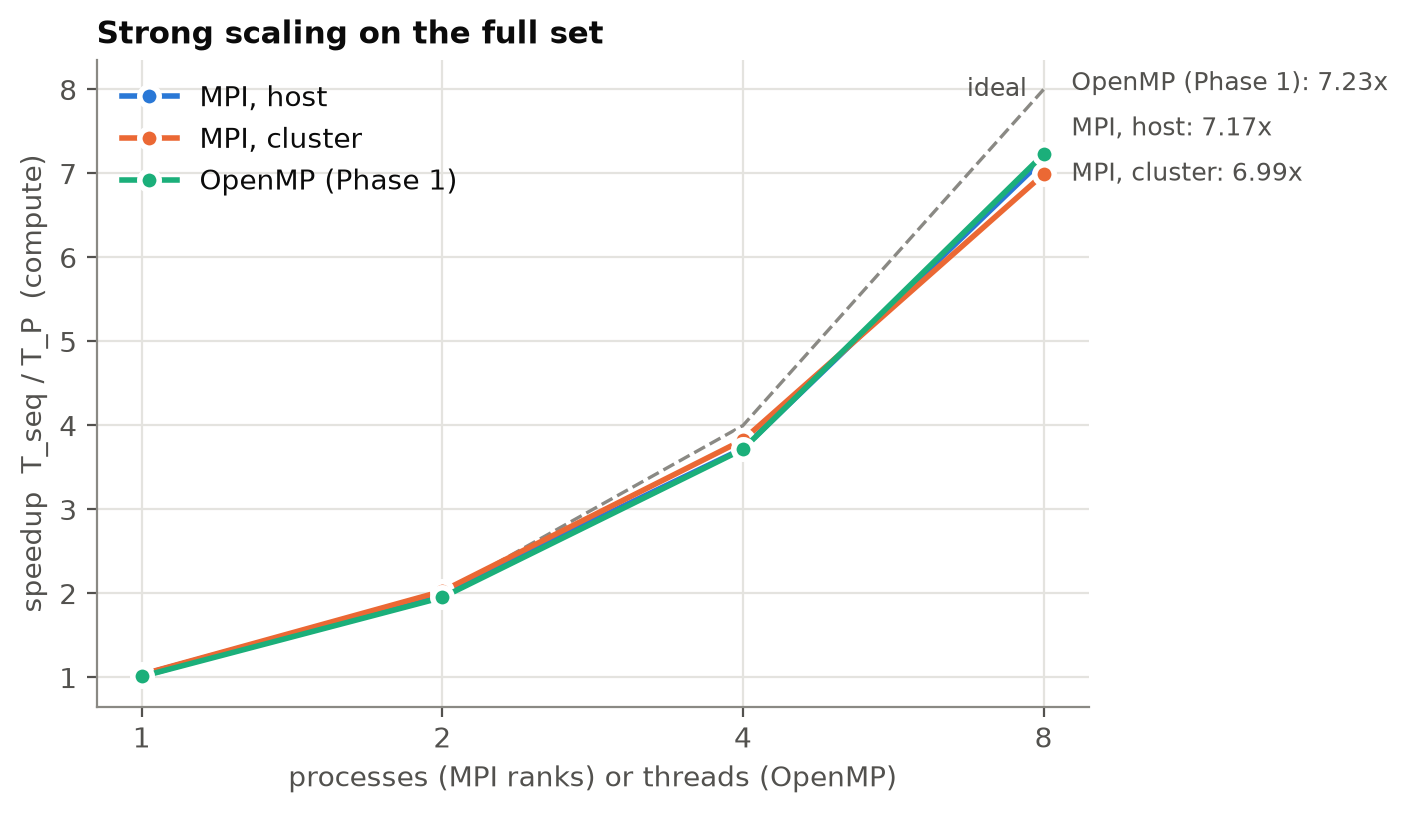
\includegraphics[width=\linewidth]{strong.png}\caption{}\end{subfigure}\hfill
\begin{subfigure}{0.49\linewidth}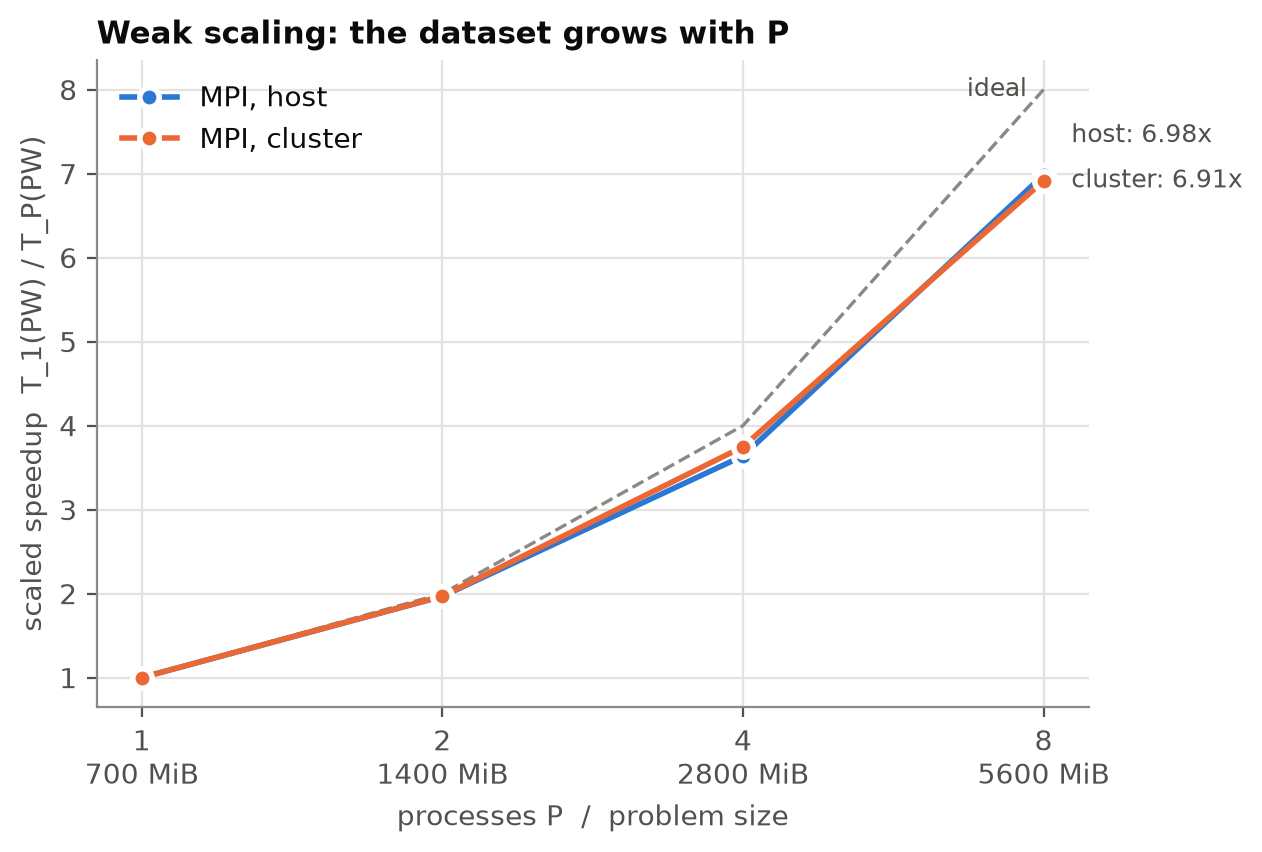
\includegraphics[width=\linewidth]{weak.png}\caption{}\end{subfigure}
\caption{(a) Strong scaling on the full set. (b) Weak scaling: $P$ ranks on $P\times700$\,MiB.}
\label{fig:scaling}
\end{figure}

\paragraph{Strong scaling.} MPI matches OpenMP in compute speedup (7.17 against 7.23 at 8), and
the cluster is within 3\,\% of the host although its ranks communicate over TCP. Both follow
from the previous section: communication is under 0.1\,\% of the run. The efficiency of 0.90 at
$P=8$ has the same cause as in Phase 1, the processor's lower clock when all cores are active,
not message passing.

\paragraph{MPI is faster end to end.} $S_\text{total}$ is 7.14 for MPI against 6.27 for OpenMP.
The OpenMP program opens and touches the whole set serially before its parallel region (0.25\,s).
Each MPI rank opens only its own part, so that step is divided by $P$ (0.04\,s at $P=8$). The
serial fraction that limited Phase 1 end to end is gone. The small sets show it most:
at $P=8$ the 500MB set reaches $S_\text{total}=7.35$ with MPI against 5.53 with OpenMP.

\paragraph{Weak scaling.} With 700\,MiB per rank, the run time grows only from 1.09\,s to
1.25\,s (host) and 1.27\,s (cluster) at $P=8$. The scaled speedup is 6.98 (host) and 6.91
(cluster), against 7.02 for OpenMP, with weak efficiency 0.87 and 0.86. The loss is again the
clock and the shared memory system of one machine, not communication, which stays constant at a
few hundred bytes per rank as the problem grows.

\paragraph{Hybrid MPI + OpenMP (bonus).} The MPI program runs OpenMP threads inside each rank
(\texttt{-t}). With 8 cores in every configuration (Table~\ref{tab:hybrid}), the compute time is
the same to within 2\,\%, as expected for independent work. The total improves with more ranks,
because start-up is parallel across ranks but serial inside one.

\begin{table}[H]
\centering\small
\begin{tabular}{lrrrr}
\toprule
Ranks $\times$ threads & $1\times8$ & $2\times4$ & $4\times2$ & $8\times1$ \\
\midrule
Compute (s) & 1.346 & 1.334 & 1.356 & 1.352 \\
Total (s) & 1.586 & 1.462 & 1.424 & 1.401 \\
$S_\text{total}$ & 6.34 & 6.88 & 7.06 & 7.18 \\
\bottomrule
\end{tabular}
\caption{Hybrid configurations on the host, full set.}
\label{tab:hybrid}
\end{table}

%======================================================================
\section{Communication overheads and challenges}
%======================================================================

\begin{itemize}
  \item \textbf{Overhead is negligible by design.} The decomposition sends 0.4\,MiB of metadata
    for 5.9\,GiB of data, in three latency-bound exchanges. The price is that every node must
    be able to read the dataset (a shared or replicated file system).
  \item \textbf{Shipping data is what costs.} As soon as tensors travel (collect mode), a
    serial receiver caps throughput at 1.9\,GiB/s, and non-blocking sends only help while the
    receiver has spare capacity.
  \item \textbf{Our cluster is not a real network.} The containers share one machine: the
    bridge has 6\,\textmu s latency and 7.6\,GB/s, far better than Ethernet, and all ``nodes''
    share one memory bus, one L3 cache and one page cache. On real nodes each message would
    cost more (latency typically tens of microseconds, bandwidth near 0.1\,GB/s on gigabit
    Ethernet), but 0.4\,MiB per run would still be negligible; the collect-mode results would
    get much worse. Real nodes would also not share the clock-frequency limit.
  \item \textbf{Process binding.} OpenMPI cannot bind ranks to cores inside CPU-restricted
    containers, so binding is off there and each container's CPU set does the pinning.
  \item \textbf{Progress of non-blocking sends.} A large \texttt{MPI\_Isend} only advances
    inside MPI calls, so overlap needs explicit \texttt{MPI\_Test} calls in the compute loop.
  \item \textbf{Verification paid off.} Because the computation is exact, any partition, rank
    count or transport must reproduce the same integers and CRCs, which made every experiment
    in this report self-checking.
\end{itemize}

\end{document}
